\documentclass[border=3pt]{standalone}
% Preâmbulo compartilhado pelos diagramas TikZ da aula 8 de IHC (Design de IHC)
\usepackage[T1]{fontenc}
\usepackage[utf8]{inputenc}
\usepackage{lmodern}
\usepackage{amsmath}
\usepackage{xcolor}
\usepackage{tikz}
\usetikzlibrary{arrows.meta,angles,quotes,decorations.pathmorphing,decorations.pathreplacing,calc,
                positioning,shapes.geometric,shapes.misc,backgrounds,fit,
                math}

% Paleta (mesma dos SVGs originais)
% Paleta da disciplina de IHC: acento roxo (#755099), da capa do livro.
% (o nome "dblue" é mantido para não alterar todos os diagramas)
\definecolor{dblue}{HTML}{755099}
\definecolor{dorange}{HTML}{B3541E}
\definecolor{dgreen}{HTML}{4A7C59}
\definecolor{dred}{HTML}{9C4B4B}
\definecolor{dcream}{HTML}{F4F1EA}
\definecolor{dshade}{HTML}{DDD7C9}

% Função gaussiana (não normalizada por padrão de escala visual)
\pgfmathdeclarefunction{gauss}{3}{%
  \pgfmathparse{1/(#3*sqrt(2*pi))*exp(-((#1-#2)^2)/(2*#3^2))}%
}

% Estilos comuns (prefixo d... para não colidir com chaves internas do pgf)
\tikzset{
  >={Stealth[length=2mm]},
  dguide/.style={gray!55, dashed, line width=0.4pt},
  daxis/.style={gray!60, line width=0.7pt, ->},
  dbody/.style={fill=black!3, draw=black!80, line width=1pt},
  dacc/.style={draw=dblue, line width=1pt},
  dlbl/.style={black!55, font=\small},
  dsub/.style={black!45, font=\footnotesize},
  dstate/.style={circle, draw=black!80, fill=dcream, line width=1pt,
                 minimum size=17mm, font=\large, inner sep=1pt},
  dobs/.style={circle, draw=black!80, fill=dshade, line width=1pt,
               minimum size=14mm, font=\large, inner sep=1pt},
  dbox/.style={rounded corners=2pt, draw=black!80, fill=dcream, line width=1pt,
               align=center, inner sep=6pt},
  dop/.style={circle, draw=black!80, fill=white, line width=1pt,
              minimum size=6mm, inner sep=0pt, font=\small},
  dtrans/.style={->, dblue, line width=1pt},
  dmeas/.style={->, dorange, line width=1pt},
  dcurve/.style={line width=1pt, dblue},
  dcurveb/.style={line width=1.4pt, dorange},
}

\begin{document}
\hyphenpenalty=10000 \exhyphenpenalty=10000 \tolerance=9999 \emergencystretch=3em
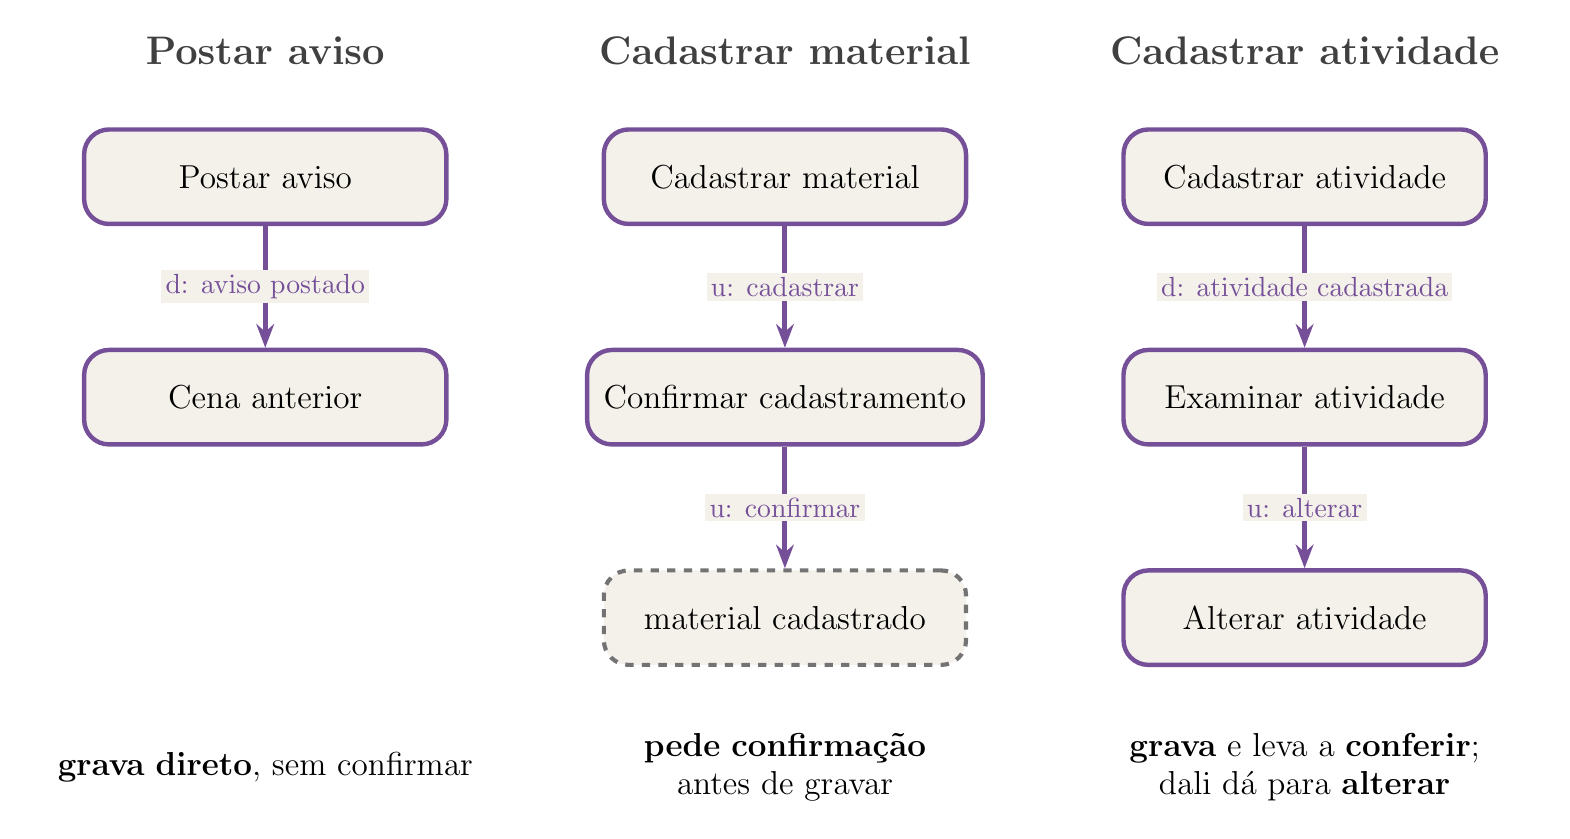
\begin{tikzpicture}[x=1cm,y=1cm]
\tikzset{s/.style={dbox, draw=dblue, rounded corners=9pt, line width=1.6pt, minimum width=4.6cm, minimum height=1.2cm, font=\large},
        r/.style={dbox, draw=black!55, dashed, rounded corners=9pt, line width=1.5pt, minimum width=4.6cm, minimum height=1.2cm, font=\large},
        a/.style={dtrans, line width=1.8pt, -{Stealth[length=3mm]}},
        l/.style={font=\normalsize, fill=dcream, inner sep=1.5pt}}
\node[font=\Large\bfseries, black!75] at (3.2,9.6) {Postar aviso};
\node[font=\Large\bfseries, black!75] at (9.8,9.6) {Cadastrar material};
\node[font=\Large\bfseries, black!75] at (16.4,9.6) {Cadastrar atividade};
% 1
\node[s] (a1) at (3.2,8.0) {Postar aviso};
\node[s] (b1) at (3.2,5.2) {Cena anterior};
\draw[a] (a1.south) -- node[l, align=center] {d: aviso postado} (b1.north);
% 2
\node[s] (a2) at (9.8,8.0) {Cadastrar material};
\node[s] (c2) at (9.8,5.2) {Confirmar cadastramento};
\node[r] (b2) at (9.8,2.4) {material cadastrado};
\draw[a] (a2.south) -- node[l] {u: cadastrar} (c2.north);
\draw[a] (c2.south) -- node[l] {u: confirmar} (b2.north);
% 3
\node[s] (a3) at (16.4,8.0) {Cadastrar atividade};
\node[s] (b3) at (16.4,5.2) {Examinar atividade};
\node[s] (c3) at (16.4,2.4) {Alterar atividade};
\draw[a] (a3.south) -- node[l, align=center] {d: atividade cadastrada} (b3.north);
\draw[a] (b3.south) -- node[l] {u: alterar} (c3.north);
\node[font=\large, text width=5.8cm, align=center] at (3.2,0.5) {\textbf{grava direto}, sem confirmar};
\node[font=\large, text width=5.8cm, align=center] at (9.8,0.5) {\textbf{pede confirmação} antes de gravar};
\node[font=\large, text width=5.8cm, align=center] at (16.4,0.5) {\textbf{grava} e leva a \textbf{conferir}; dali dá para \textbf{alterar}};
\end{tikzpicture}
\end{document}
